% To je predloga za poročila o domačih nalogah pri predmetih, katerih
% nosilec je Blaž Zupan. Seveda lahko tudi dodaš kakšen nov, zanimiv
% in uporaben element, ki ga v tej predlogi (še) ni. Več o LaTeX-u izveš na
% spletu, na primer na http://tobi.oetiker.ch/lshort/lshort.pdf.
%
% To predlogo lahko spremeniš v PDF dokument s pomočjo programa
% pdflatex, ki je del standardne instalacije LaTeX programov.

\documentclass[a4paper,11pt]{article}
\usepackage{a4wide}
\usepackage{fullpage}
\usepackage[utf8x]{inputenc}
\usepackage[slovene]{babel}
\selectlanguage{slovene}
\usepackage[toc,page]{appendix}
\usepackage[pdftex]{graphicx} % za slike
\usepackage{setspace}
\usepackage{color}
\definecolor{light-gray}{gray}{0.95}
\usepackage{listings} % za vključevanje kode
\usepackage{hyperref}
\usepackage{subfig}
\usepackage{titlesec}
\usepackage{flafter}
\renewcommand{\baselinestretch}{1.2} % za boljšo berljivost večji razmak
\renewcommand{\appendixpagename}{\normalfont\Large\bfseries{Priloge}}


\titleformat{name=\section}[runin]
  {\normalfont\bfseries}{}{0em}{}
\titleformat{name=\subsection}[runin]
  {\normalfont\bfseries}{}{0em}{}


% header
\makeatletter
\def\@maketitle{%
  \noindent
  \begin{minipage}{2in}
  \@author
  \end{minipage}
  \hfill
  \begin{minipage}{1.2in}
  \textbf{\@title}
  \end{minipage}
  \hfill
  \begin{minipage}{1.2in}
  \@date
  \end{minipage}
  \par
  \vskip 1.5em}
\makeatother


\lstset{ % nastavitve za izpis kode, sem lahko tudi kaj dodaš/spremeniš
language=Python,
basicstyle=\footnotesize,
basicstyle=\ttfamily\footnotesize\setstretch{1},
backgroundcolor=\color{light-gray},
}


% Naloga
\title{Naloga 4}
% Ime Priimek (vpisna)
\author{Andrej Hafner (63160122)}
\date{\today}

\begin{document}

\maketitle


\normalfont\textsl{}
\section{Regularizacija.}Vpliv regularizacije na klasifikacijo z logistično regresijo pri različnih vrednostih parametra $\lambda$. 
\begin{figure}%
	
	\centering
	\subfloat{{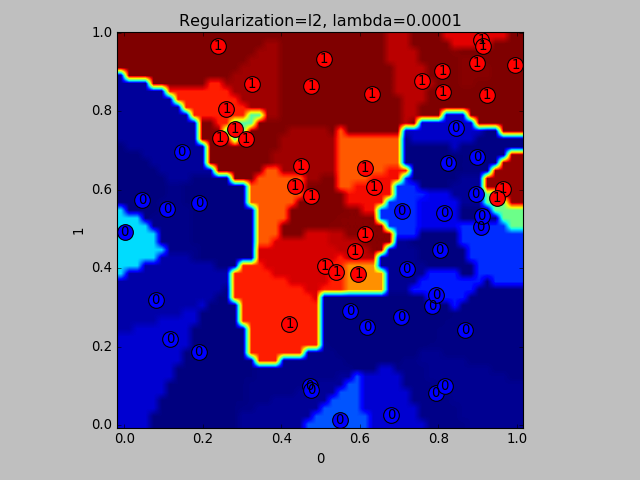
\includegraphics[clip,width=5cm]{myplot2}}}%
	
	\qquad

	\subfloat{{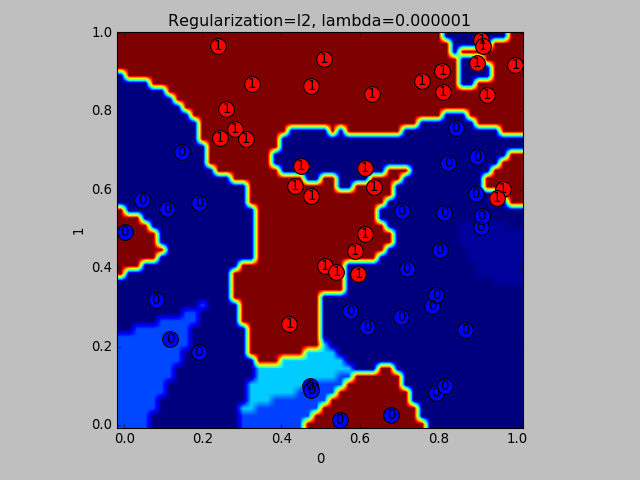
\includegraphics[clip,width=5cm]{myplot3}}}%

\end{figure}
\begin{figure}[!htb]
\centering
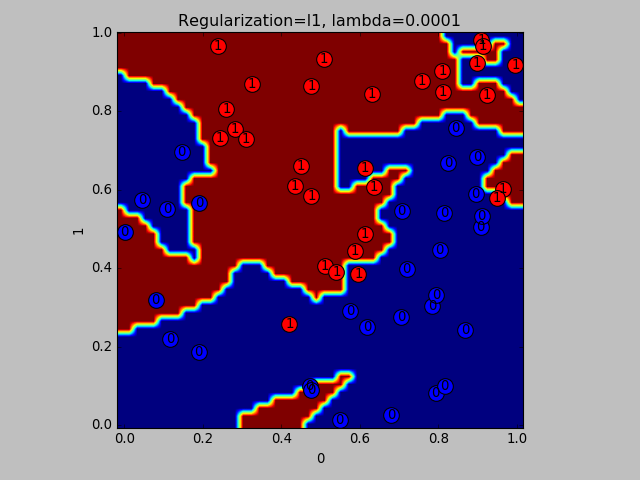
\includegraphics[clip,scale=0.35]{myplot4}
\end{figure}
\pagebreak

	

\section{Točnosti.} Primerjava različnih stopenj regularizacije pri testiranju na vseh učnih podatkih in pri prečnem preverjanju.
\begin{table}[htbp]
	\caption{Vrednost parametra $\lambda$ in napovedna točnost pri prečnem preverjanju, ter testiranju na učnih podatkih.}
	\label{tab1}
	\begin{center}
		\begin{tabular}{llp{4.3cm}}
			\hline
			 $\lambda$ & CA (učni podatki) & CA (prečno preverjanje) \\
			\hline
			$10^{-10}$ & 1.00  & 0.80 \\
			$10^{-9}$ & 1.00  & 0.78 \\
			$10^{-8}$ & 1.00  & 0.78 \\
			$10^{-7}$ & 1.00  & 0.78 \\
			$10^{-6}$ & 1.00  & 0.78 \\
			$10^{-5}$ & 1.00  & 0.78 \\
			$10^{-4}$ & 1.00  & 0.77 \\
			$10^{-3}$ & 1.00  & 0.73 \\
			$10^{-2}$ & 1.00  & 0.75 \\
			$10^{-1}$ & 0.96  & 0.77 \\
			$1$ & 0.95  & 0.75\\
			$10$ & 0.92  & 0.73\\
			$10^2$ & 0.88  & 0.48 \\
			$10^3$ & 0.77  & 0.50 \\
			$10^4$ & 0.77  & 0.50 \\
			\hline
		\end{tabular}
	\end{center}
\end{table}





\section{Izjava o izdelavi domače naloge.}
Domačo nalogo in pripadajoče programe sem izdelal sam.


\end{document}
